\chapter{Relational DataBase Management Systems (RDBMS)}

\section{PostgreSQL}\label{sec:postgresql}

We will focus on PostgreSQL as our primary database, so this chapter is written within that context.
Later on we will introduce other non-relational technologies.
Reasons for choice of PostgreSQL:

\begin{itemize}
\item
  It is free software and can be installed on any operating system.
\item
  No limits / free-trial limitations.
\item
  Support exists for geospatial data, JSON, XML, full-text search etc.
\item
  Has some support for masquerading as other types of DB (e.g. graph data).
\end{itemize}

You should bookmark the
\href{https://www.postgresql.org/docs/13/}{PostgreSQL} documentation.

As we continue we will refer to PostgreSQL as Postgres for brevity.


\section{Query Language}

ANSI standardised SQL but most Databases use a derived form of it. 

PostgreSQL uses a dialect of SQL.

We can interact with PostgreSQL using any client program that implements the PostgreSQL protocol.
The simplest is the \texttt{psql} client. 


\section{Relational data structure}

On a single host, a relational database management system \textbf{cluster} provides one or more isolated \textbf{databases}.
Within a database, data is contained in one or more \textbf{tables} according to the \textbf{schema}.
\autoref{fig:rdbms-terms} shows the key relational data structure:

\begin{figure}[htbp]
  \centering
  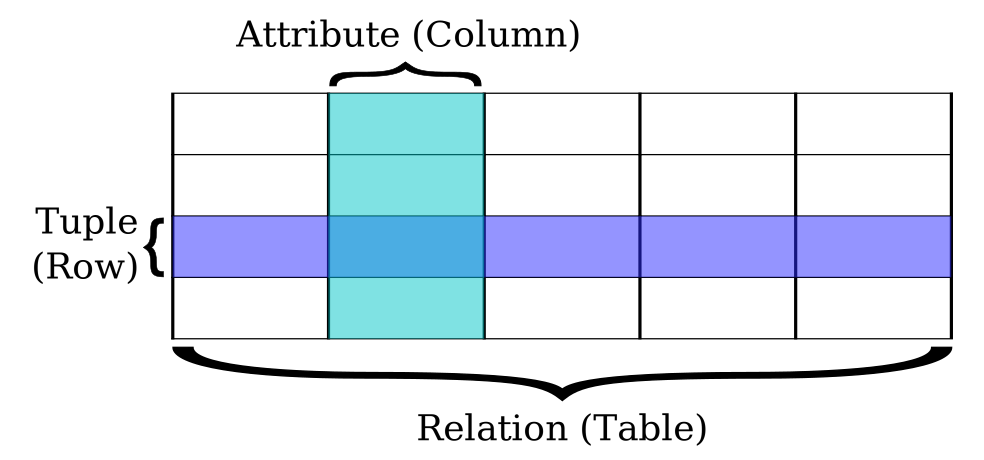
\includegraphics[width=0.5\linewidth]{rdbms_terms}
  \caption{Relational model terminology}
  \label{fig:rdbms-terms}
\end{figure}

\begin{description}
\item[Relation (Table):] with columns and rows. Table names must be unique.
\item[Attribute (Column):] holding distinct part of a row: 
  \begin{itemize}
  \item Column has a \textbf{data type} (e.g. integer, text) from an allowable list (database-dependent).
    \begin{itemize}
    \item We can define our own data types for consistency throughout a database.
    \end{itemize}
  \item Column may allow / permit \textbf{null} values (unknown, empty, undefined, blank)
  \item Column order has no meaning or significance.
  \end{itemize}
\item[Tuple (Row):] a single record contained with a table.
  \begin{itemize}
  \item No theoretical upper limit on number of rows.
  \item The natural order of rows in a table is meaningless!  Do not rely on it!
  \end{itemize}
\end{description}

\subsection{Null values}

Null denotes a lack of a value, used to indicate that data is missing, unknown, blank, undefined:
\begin{itemize}
\item Null is \textbf{not} zero, the empty string, false or any other value.
\item Null values will pollute other expressions (e.g. arithmetic, comparison)
  \begin{itemize}
  \item Null does not even equal null!
  \end{itemize}
\item Can test for null with \texttt{IS NULL} operation.
\end{itemize}
While the concept of null can be confusing, it's actually very useful.
It avoids placeholder or marker data.
Specifically testing for it allows unknown values to be treated differently. 

\subsection{Unique constraints}

Within a table, a unique constraint on a column or group of columns will prevent duplicate rows existing.  

\subsection{Primary key}

Practically we need ways to identify any row individually.
Within any table, there may be a number of \textbf{candidate keys} that could be used to identify each row.
\begin{description}
\item[Simple key:] a single column that is:
  \begin{description}
  \item[not null] so that every row can be identified.
  \item[unique] so that every row is distinct. 
  \end{description}
\item[Complex key:] two or more columns:
  \begin{enumerate}
  \item no columns in the key are null
  \item together are unique
  \end{enumerate}
\end{description}
For each table, one of its candidate keys is selected as the \textbf{primary key}.
This is normally encoded explicitly by DML in the database.


\subsection{Foreign key}

The foreign key is one of the most powerful mechanisms in relational databases.
It allows us to explicitly encode the idea of a table being linked to another.

A foreign key defined on a column points to a column (usually the primary key) of another table.

The RDBMS enforces the constraint that a value in the foreign key column must exist in the referenced table.
We will meet foreign keys again when we set up multi-table databases.



\section{Defining characteristics}

Codd's Seminal paper defines a number of characteristics that a relational database must possess.

\subsection{Foundation rule}
  For any system that is advertised as, or claimed to be, a relational database management system, that system must be able to manage databases entirely through its relational capabilities.
  
\subsection{Information Rule}
  All information in a relational database is represented explicitly at the logical level and in exactly one way --- by values in tables.

\subsection{Guaranteed access rule}
  Each and every datum (atomic value) in a relational database is guaranteed to be logically accessible by resorting to a combination of table name, primary key value and column name.

\subsection{Systematic treatment of null values}
  Null values (distinct from the empty character string or a string of blank characters and distinct from zero or any other number) are supported in fully relational DBMS for representing missing information and inapplicable information in a systematic way, independent of data type.

\subsection{Dynamic online catalog based on the relational model}
  The database description is represented at the logical level in the same way as ordinary data, so that authorized users can apply the same relational language to its interrogation as they apply to the regular data.

\subsection{Comprehensive data sublanguage rule}
  A relational system may support several languages and various modes of terminal use (for example, the fill-in-the-blanks mode). However, there must be at least one language whose statements are expressible, per some well-defined syntax, as character strings and that is comprehensive in supporting all of the following items:
  \begin{enumerate}
  \item Data definition.
  \item View definition.
  \item Data manipulation (interactive and by program).
  \item Integrity constraints.
  \item Authorization.
  \item Transaction boundaries (begin, commit and rollback). \textit{We will meet transactions again later on.}
  \end{enumerate}

\subsection{View updating rule}
  All views that are theoretically updatable are also updatable by the system.

\subsection{Relational Operations Rule / Possible for high-level insert, update, and delete}
  The capability of handling a base relation or a derived relation as a single operand applies not only to the retrieval of data but also to the insertion, update and deletion of data.

\subsection{Physical data independence}
  Application programs and terminal activities remain logically unimpaired whenever any changes are made in either storage representations or access methods.

\subsection{Logical data independence}:
  Application programs and terminal activities remain logically unimpaired when information-preserving changes of any kind that theoretically permit unimpairment are made to the base tables.

\subsection{Integrity independence}
  Integrity constraints specific to a particular relational database must be definable in the relational data sublanguage and storable in the catalog, not in the application programs.
  
\subsection{Distribution independence}
  The end-user must not be able to see that the data is distributed over various locations. Users should always get the impression that the data is located at one site only.

\subsection{Non-subversion rule}
  If a relational system has a low-level (single-record-at-a-time) language, that low level cannot be used to subvert or bypass the integrity rules and constraints expressed in the higher level relational language (multiple-records-at-a-time).



